%\documentclass[12pt,a4paper]{report}
\documentclass{standalone}

\usepackage[italian]{babel}
\usepackage{newlfont}
\usepackage{color}
\usepackage[utf8]{inputenc}
\usepackage{eurosym}
\usepackage{graphicx}
\usepackage{fancyhdr}
\usepackage{subfig}
\usepackage{subfloat}
\usepackage{subcaption}
\textwidth=450pt\oddsidemargin=0pt
\renewcommand{\baselinestretch}{1.4}
\makeindex


\begin{document}
	\pagestyle{fancy}
	\lhead{\rightmark}
	\rhead{\thepage}

\chapter{Introduzione}
Lo scopo dell'esperimento è quello di misurare il tempo di vita media dei muoni generati dall'interazione dei raggi cosmici con l'atmosfera (1.1). I muoni sono leptoni carichi che decadono debolmente (1.3) e, essendo MIP (Minimum Ionizing Particles), riescono ad attraversare grandi quantità di materiale (1.2). Il tempo di vita media misurato è quello relativo al decadimento di muoni a riposo, che devono quindi essere fermati all'interno dell'apparato (1.4)

\section{I raggi cosmici}
I raggi cosmici (RC) sono nuclei altamente ionizzanti accelerati da sorgenti astrofisiche che giungono sulla Terra in maniera isotropa. La composizione chimica dei RC è molto simile a quella del Sistema Solare, il che significa che vi sono presenti nuclei di idrogeno ed elio in abbondanza, ma anche, in misura minore,  tutti i nuclei fino al ferro.
I RC primari hanno uno spettro di energie molto ampio che va da una frazione di Gev fino a $10^{11}$ Gev il che li rende le particelle più energetiche misurabili in Fisica (al Large Hadron Collider del CERN si raggiungono energie di 7 Tev).
Una volta entrati in contatto con i nuclei dell'atmosfera i RC interagiscono con essi generando degli sciami di particelle principalmente composti da $\pi^\pm, \pi^0$ \cite{Spurio}.
I pioni neutri decadono quasi istantaneamente ($\tau \sim 10^{-17}$ s) in due fotoni, mentre i pioni carichi decadono quasi esclusivamente (BR = 99.98770 $\pm$ 0.00004) in muone e neutrino muonico.
I fotoni $prompt$ derivanti dal decadimento del $\pi^0$, interagendo con i nuclei dell'atmosfera, producono coppie $e^+e^-$ di alta energia che a loro volta emetteranno fotoni per bremsstrahlung e così via, generando uno sciame elettromagnetico.

A differenza degli elettroni i muoni, essendo MIP (Minimum Ionizing Particle), interagiscono molto debolmente con i nuclei dell'atmosfera e rappresentano quindi, insieme ai neutrini, la componente più penetrante dei RC. In Fig 1.1 si riporta uno schema dell'interazione dei RC con l'atmosfera. 

\begin{figure}[H]
	\centering
	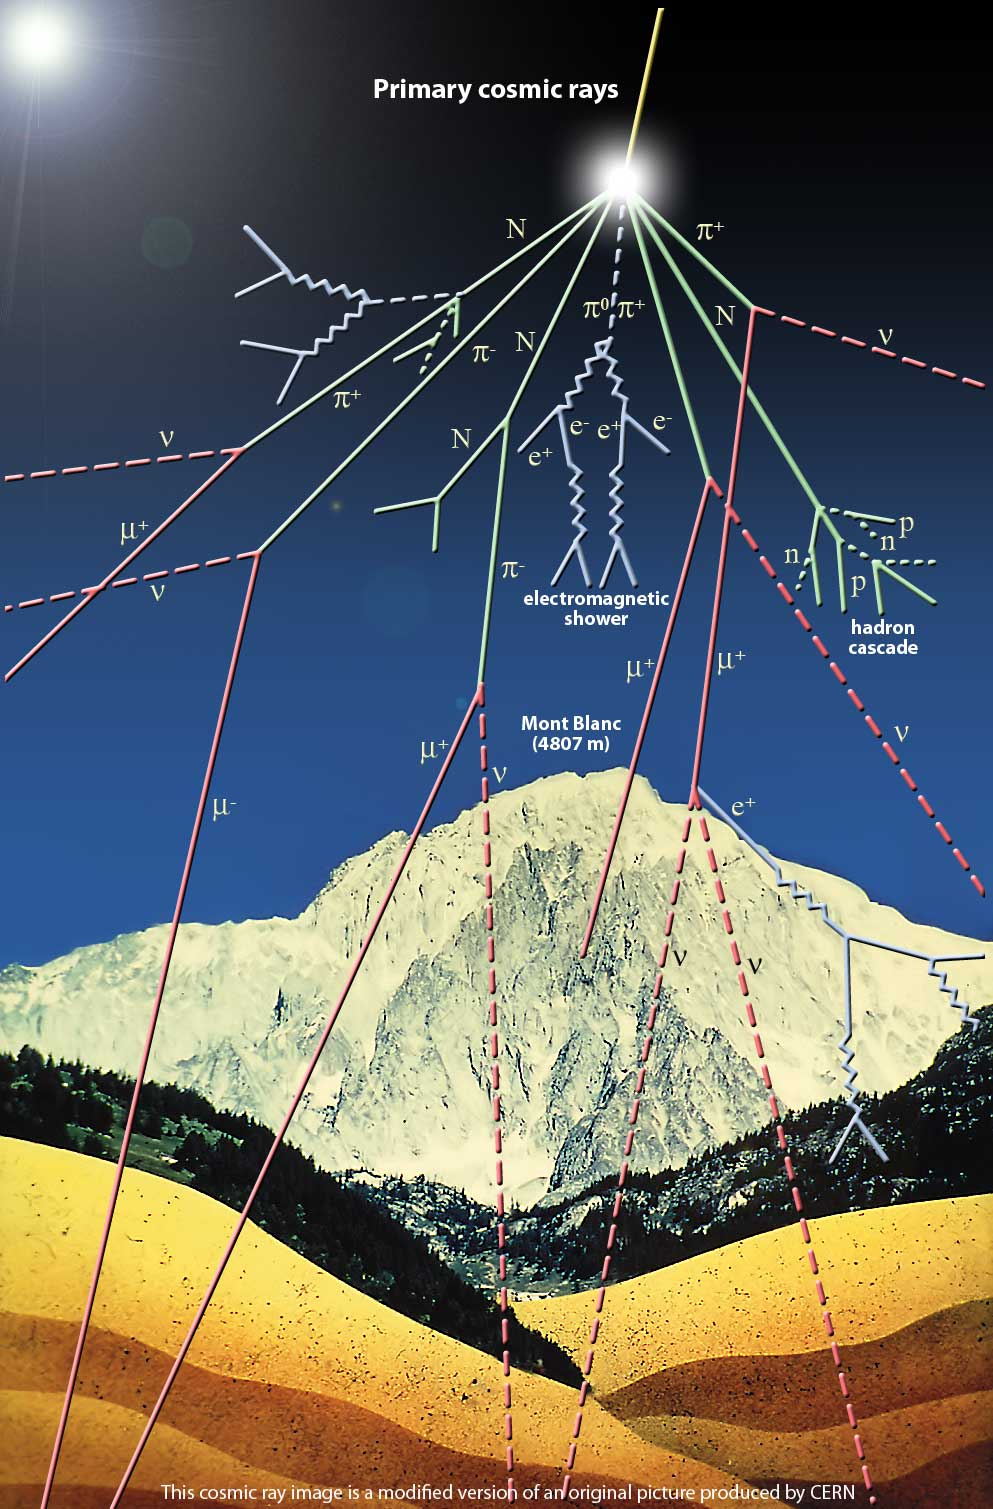
\includegraphics[width=6.5cm, height=10cm]{images/cosmic-rays.jpg}
	\caption{Sciami prodotti in atmosfera dai raggi cosmici}
\end{figure}


Il flusso di muoni al livello del mare varia con l'energia con una legge del tipo $\Phi_\mu \propto KE^{-2.7}$ dove $K$ è una costante; l'energia media dei muoni che arrivano sulla superficie terrestre è $<E>_\mu \approx 4$ GeV. 
\clearpage
\section{Interazioni con la materia}
I muoni sono leptoni carichi come gli elettroni ed anche loro interagiscono con la materia tramite ionizzazione o, ad energie più elevate, tramite bremsstrahlung.
I muoni sono però dotati di una massa 200 volte superiore a quella degli elettroni, il che rende l'energia critica (energia alla quale la probabilità di perdere energia per ionizzazione eguaglia quella di perderla per bremsstrahlung) molto più elevata.
Come si può notare dalla Fig.1.2 i muoni sono particelle al minimo di ionizzazione per energie inferiori al TeV \cite{Groom}.
\begin{figure}[H]
	\centering
	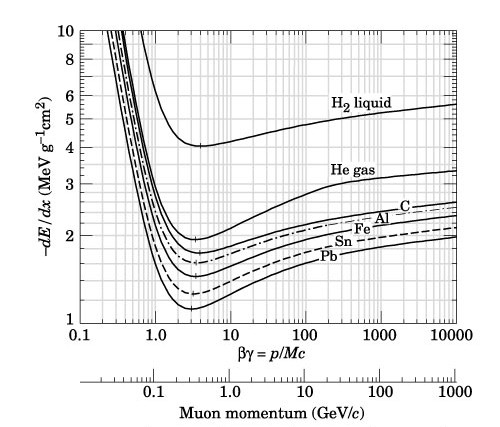
\includegraphics[width=9cm, height=7.5cm]{images/Energyloss.jpg}
	\caption{Perdita di energia per ionizzazione dei muoni in diversi materiali}
\end{figure}
A basse energie il ${\mu}^-$ ha inoltre la possibilità di venire catturato da un nucleo generando un atomo muonico.
Tale stato legato modifica la vita media del muone di una quantità che varia a seconda del tipo di nucleo.
\section{Decadimento del muone}
Il muone decade debolmente con un BR $\approx$ 100$\%$ nel canale elettronico secondo la reazione (per l'antimuone la reazione di decadimento è la coniugata di carica):\\
\centerline{$\mu^- \rightarrow e^- \nu_\mu \bar{\nu_e}$}
Essendo la probabilità di decadimento per unità di tempo costante, la probabilità che un muone generato al tempo $t=0$ sopravviva fino al tempo $t$ è di tipo poissoniano:\\
\centerline{$P(t)=e^{-t/\tau_\mu}$}
dove $\tau_\mu$ indica la vita media del muone nel sistema di riferimento solidale con esso.
Da tale probabilità si ottiene, per un insieme di particelle, la ben nota legge del decadimento esponenziale: \cite{Bendiscioli} \\
\centerline{$N(t)=N_0e^{-t/\tau_\mu}$}

\section{Apparato sperimentale}
L'appartato sperimentale utilizzato per effettuare le misure è composto da un blocco di ferro spesso 26 cm seguito da due piani di scintillatore plastico (denominati Piano 0 e Piano 1) sotto cui sono poste una lastra di ferro di 0.5 cm di spessore e un terzo piano di scintillatore (Piano 2).
Ogni piano di scintillatore è composto da due semipiani (0 e 1), secondo la convezione per cui il semipiano 0 è quello posto nel lato frontale del rivelatore. Ai capi di ogni semipiano sono posti tre fotomoltiplicatori accoppiati in un unico tripletto, per un totale di 12 tripletti. Nel seguito di tale lavoro sarà denominato un tripletto di PMT indicando il semipiano di scintillatore a cui è accoppiato e il lato su cui è collegato (Left o Right); ad esempio P01R indica il tripletto collegato al lato destro del secondo semipiano del Piano 0.
In Fig 1.3 è riportata una vista frontale del rivelatore mentre in Fig 1.4 una vista laterale.

\begin{figure}[H]
	\centering
  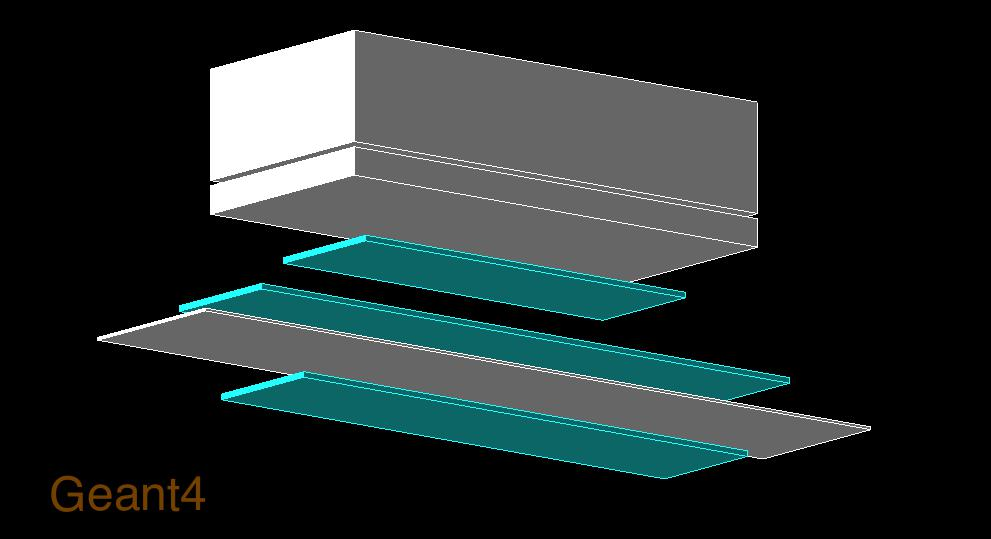
\includegraphics[width=12cm, height=7.5cm]{images/general.jpg}
  \caption{Simulazione dell'apparato utilizzato realizzata con le librerie grafiche di Geant4.}
\end{figure}

\begin{figure}[H]
  \centering
  \subfloat[][]{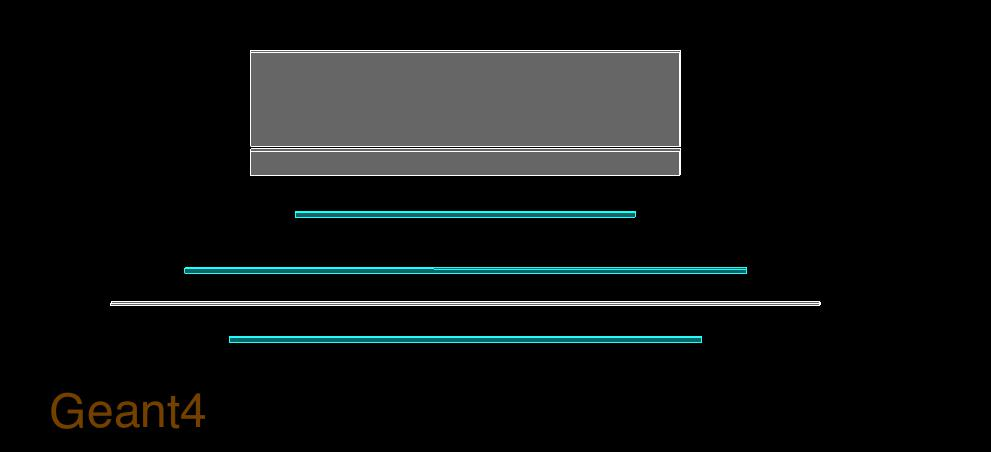
\includegraphics[width=.8\textwidth]{images/frontale.jpg}\label{frontal}}\\
  \subfloat[][]{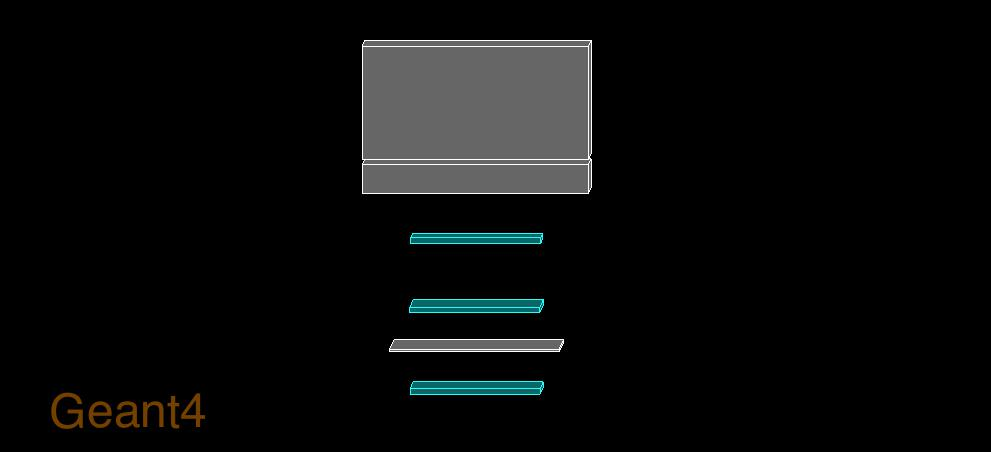
\includegraphics[width=.8\textwidth]{images/laterale.jpg}\label{lateral}}\\
  \subfloat[][]{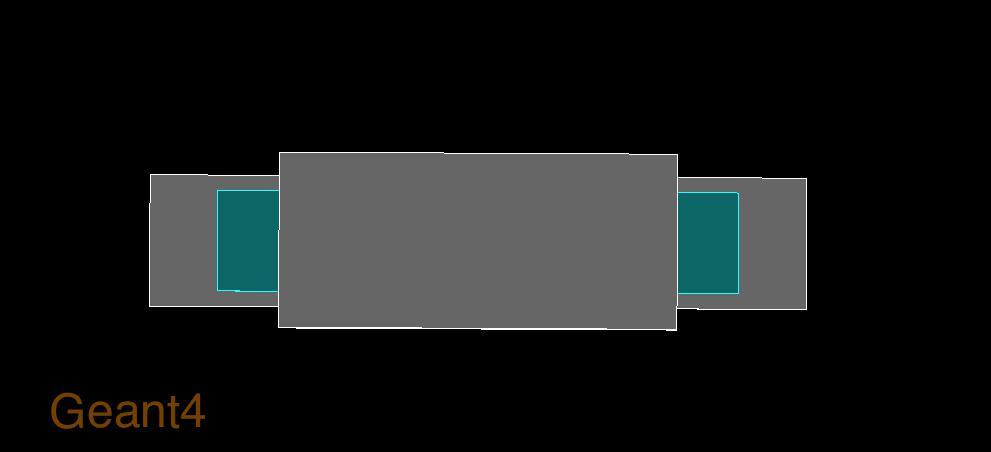
\includegraphics[width=.8\textwidth]{images/sopra.jpg}\label{up}}\\
  \subfloat[][]{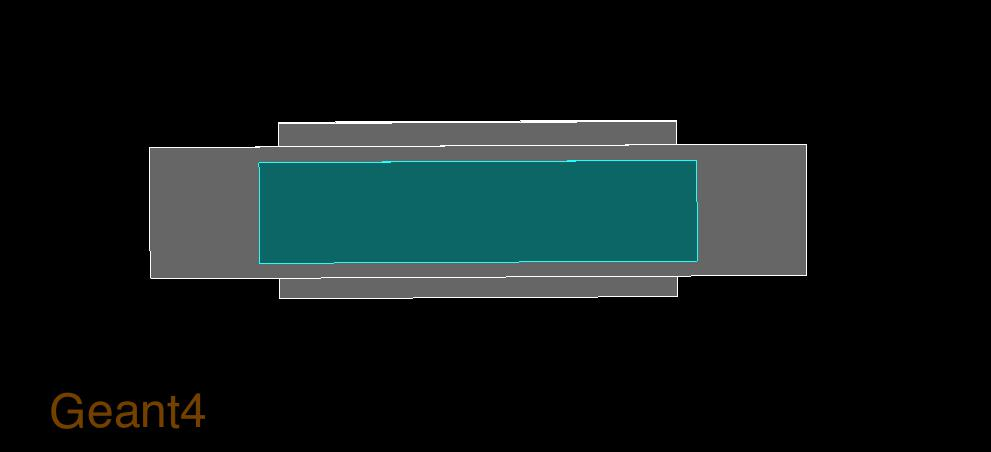
\includegraphics[width=.8\textwidth]{images/sotto.jpg}\label{down}}\\
  \caption{Simulazione del rivelatore da varie angolazioni.}
  \label{fig:detector_sides}
\end{figure}

Il blocco di ferro posto sopra il rivelatore serve per schermare eventuali elettroni o positroni provenienti dai RC e permettere il passaggio ai soli muoni.
Al fine di misurare il tempo di vita media del muone nel sistema di riferimento solidale con esso è necessario che il muone venga fermato dalla lastra di ferro prima di decadere. Selezionando questa classe di eventi particolare, denominata nel seguito del lavoro $\mu_{stop}$, è possibile misurare il tempo proprio di decadimento, evitando una dilatazione nella misura data dal fattore di Lorentz $\gamma$.

Gli eventi $\mu_{stop}$ vengono selezionati costruendo un circuito di trigger che individua le sole particelle che danno un segnale nel Piano 0 e nel Piano 1, ma non nel Piano 2 (cfr Misure Preliminari/Trigger). In questo modo è idealmente possibile selezionare i muoni che, dopo essere stati rallentati dal blocco di ferro, attraversano i primi due scintillatori e vengono fermati dalla lastra di ferro dove, successivamente, decadranno.
Tale segnale di trigger viene utilizzato come start per i TDC che verranno poi stoppati da un segnale rivelato su uno dei tre piani, idealmente generato dall'elettrone. Dalla distribuzione dei tempi di decadimento misurati è infine possibile, tramite un fit esponenziale, ricavare la vita media del muone.

Un'altra categoria di eventi utilizzata per la misura di perdita di energia (cfr Appendice) è quella dei $\mu_{passante}$ ovvero dei muoni che attraversano tutte le tre lastre di scintillatore. In Fig. 1.5 è mostrato uno schema del rivelatore visto lateralmente dove sono idealizzate le due categorie di eventi presi in esame.

\begin{figure}[H]
	\centering
  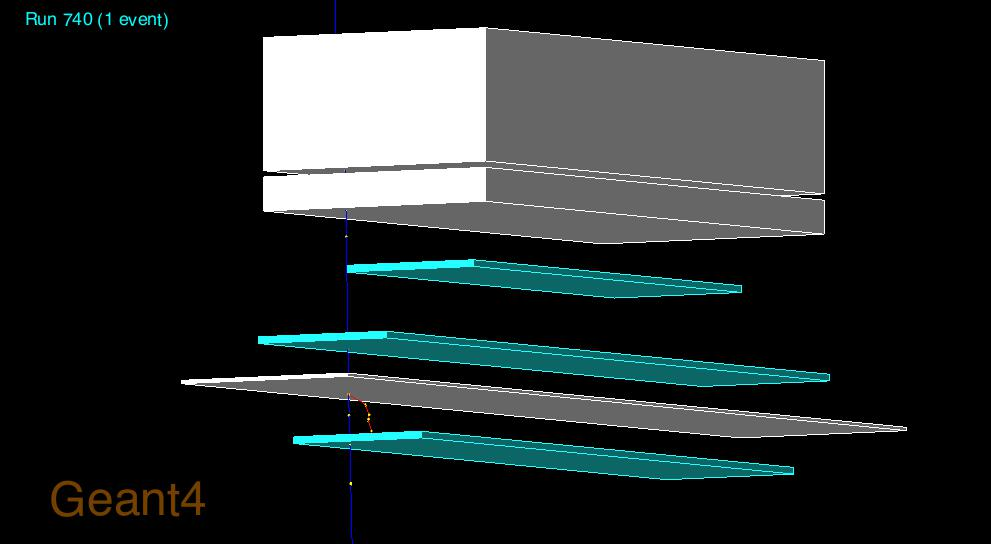
\includegraphics[width=13cm, height=7.5cm]{images/mu_stop.jpg}
	\caption{Schematizzazione degli eventi $\mu_{stop}$ e $\mu_{through}$ nel rivelatore}
\end{figure}


\end{document}
